\documentclass[11pt,a4paper]{exam}

\usepackage{listings}% C++ & Java
\usepackage{xcolor} % for setting colors
\usepackage{amsmath,amsthm,amsfonts,amssymb,dsfont,mathrsfs}
\usepackage{mathtools}
\usepackage{mathdesign}
\usepackage{textcomp}
\usepackage{ifthen}
\usepackage{tikz}
\usepackage{tkz-graph}
\usepackage[top=3cm,right=1.5cm,bottom=3cm,left=1.5cm]{geometry} 
%%%%%%%%%%Matrix Package
\usepackage{nicematrix}

%%%%%%%                                                                                                                         Table Package%%
\usepackage{tabularx}
\usepackage{multirow}
\usepackage{hhline}
%%%%%%%%%%%%%%%%%
\usepackage{hyperref}

\usepackage{color,graphicx}

\usepackage[Kashida]{xepersian}

%%%%%%%%%%%%%%%
%پکیج الگوریتم 
\usepackage{algpseudocode}
\usepackage{algorithmicx}
%%%%%%






%%%%%%%
\algrenewcommand\algorithmicwhile{\textbf{am\’\i g}}
\algrenewcommand\algorithmicdo{\textbf{v\’egezd el}}
\algrenewcommand\algorithmicwhile{\textbf{am\’\i g}}
\algrenewcommand\algorithmicdo{\textbf{v\’egezd el}}
\algrenewtext{EndWhile}{\algorithmicwhile\ \algorithmicend}
\algnewcommand\algorithmicto{\textbf{to}}
\algsetblock[<block>]{<start>}{<end>}
{<lifetime>}{<indent>}
\algnotext[<block>]{<ending command>}
%%%%%%%%%% C++ & Java Style
% set the default code style
\lstset{
% frame=(none|leftline|topline|bottomline|lines|single|shadowbox)
% frameshape={(top shape)}{(left shape)}{(right shape)}{(bottom shape)}
    frame=none,% frame=none, %  (frame=tb draw a frame at the top and bottom of the code block)
    tabsize=4, % tab space width
    showstringspaces=false, % don't mark spaces in strings
    numbers=none, % display line numbers on the left
    commentstyle=\color{green}, % comment color
    keywordstyle=\color{blue}, % keyword color
    stringstyle=\color{red} % string color
}

%%%%%%%%%%%%%%% Font Setting 
\settextfont[Scale=1.1]{XB Niloofar}
\setlatintextfont[Scale=1.1]{Times New Roman}
\setdigitfont[Scale=1.1]{Persian Modern}

%%%%%%%%%%%%%%%newtheorems
\theoremstyle{definition}
\newtheorem{thm}{قضیه}
\newtheorem{cor}[thm]{نتیجه}
\newtheorem{lem}[thm]{لم}
\newtheorem{prop}[thm]{گزاره}
\newtheorem*{exm}{مثال}
\newtheorem*{defi}{تعریف}
\newtheorem{point}[thm]{نکته}
\newtheorem{ex}[thm]{تمرین}
\newtheorem{remark}[thm]{تذکر}
\newtheorem{qarardad}[thm]{قرارداد}
%%%%%%newcommands for newtheorems
\newcommand{\bt}{\begin{thm}}
\newcommand{\et}{\end{thm}}
\newcommand{\bl}{\begin{lem}}
\newcommand{\el}{\end{lem}}
\newcommand{\bpr}{\begin{prop}}
\newcommand{\epr}{\end{prop}}
\newcommand{\bc}{\begin{cor}}
\newcommand{\ec}{\end{cor}}
\newcommand{\bp}{\begin{proof}}
\newcommand{\ep}{\end{proof}}
\newcommand{\be}{\begin{exm}}
\newcommand{\ee}{\end{exm}}
\newcommand{\bex}{\begin{ex}}
\newcommand{\eex}{\end{ex}}
\newcommand{\bd}{\begin{defi}}
\newcommand{\ed}{\end{defi}}
\newcommand{\br}{\begin{remark}}
\newcommand{\er}{\end{remark}}
\newcommand{\bq}{\begin{qarardad}}
\newcommand{\eq}{\end{qarardad}}
%%%%%%%%%%%%%%%Folder for images
\graphicspath{ {Images/} }
%%%%%%%%%%%%%%%New Operators
\newcommand{\adj}{\mathrm{adj}}
\newcommand{\cof}{\mathrm{cof}}
\newcommand{\rank}{\mathrm{Rank}}
\newcommand*{\tempa}{\multicolumn{1}{|c}{}}
%%%%%%%%%%%Other commands
%تعیین فاصله خطوط
\renewcommand{\baselinestretch}{1.7}
%تعیین تورفتگی ابتدای پاراگراف
\parindent=0pt
%%%%%%%%%%%%%%%%%%%


%%%%%%%%%%%%%%%%
% دستورهایی برای سفارشی کردن سربرگ صفحات
\csname@twosidetrue\endcsname
%%%%%%%%%%%%%%%%
%دستورهایی برای هدر و فوتر
\pagestyle{headandfoot}
%%%%%%Header
\firstpageheadrule
\firstpageheader{۶/۱۰/ 1396}{ترم تحصیلی اول-۹۶-۹۷}{طراحی الگوریتمها}
\runningheadrule
\runningheader{۶/۱۰/ ۱۳۹۶}{ترم تحصیلی ۱-۹۷-۹۶, صفحه \thepage\ از \numpages}{طراحی الگوریتمها }
%%%%%%Footer
\firstpagefootrule
\firstpagefooter{صفحه \thepage\ از \numpages}{نيمسال اول 97-1396}{6/10/1396}
\runningfootrule
\runningfooter{صفحه \thepage\ از \numpages}{نيمسال اول 97-1396}{6/10/1396}

%%%%%%%%%%%%%%%%%%%
% Accumulate the answers.
\newbox\allanswers
\setbox\allanswers=\vbox{}

\newenvironment{answer}
{%
    \global\setbox\allanswers=\vbox\bgroup
    \unvbox\allanswers
}%
{%
    \bigbreak
    \egroup
}

\newcommand{\showallanswers}{\par\unvbox\allanswers}
% End Phil's answer


% Is there a better way?
\newcommand*{\getanswer}[5]{%
    \ifthenelse{\equal{#5}{a}}
    {\begin{answer}\thequestion. (الف)~#1\end{answer}}
    {\ifthenelse{\equal{#5}{b}}
        {\begin{answer}\thequestion. (ب)~#2\end{answer}}
        {\ifthenelse{\equal{#5}{c}}
            {\begin{answer}\thequestion. (ج)~#3\end{answer}}
            {\ifthenelse{\equal{#5}{d}}
                {\begin{answer}\thequestion. (د)~#4\end{answer}}
                {\begin{answer}\textbf{\thequestion. (#5)~Invalid answer choice.}\end{answer}}}}}
}

\setlength\parindent{0pt}
%usage \choice{ }{ }{ }{ }
%(A)(B)(C)(D)
\newcommand{\fourch}[5]{
    \par
    \begin{tabular}{*{4}{@{}p{0.23\textwidth}}}
        (الف)~#1 & (ب)~#2 & (ج)~#3 & (د)~#4
    \end{tabular}
    \getanswer{#1}{#2}{#3}{#4}{#5}
}

%(A)(B)
%(C)(D)
\newcommand{\twoch}[5]{
    \par
    \begin{tabular}{*{2}{@{}p{0.48\textwidth}}}
        (الف)~#1 & (ب)~#2
    \end{tabular}
    \par
    \begin{tabular}{*{2}{@{}p{0.48\textwidth}}}
        (ج)~~~#3 & (د)~~~#4
    \end{tabular}
    \getanswer{#1}{#2}{#3}{#4}{#5}
}

%(A)
%(B)
%(C)
%(D)
\newcommand{\onech}[5]{
    \par
    (الف)~#1 \par (ب)~~#2 \par (ج)~~#3 \par (د)~~#4
    \getanswer{#1}{#2}{#3}{#4}{#5}
}

\newlength\widthcha
\newlength\widthchb
\newlength\widthchc
\newlength\widthchd
\newlength\widthch
\newlength\tabmaxwidth

\setlength\tabmaxwidth{0.96\textwidth}
\newlength\fourthtabwidth
\setlength\fourthtabwidth{0.25\textwidth}
\newlength\halftabwidth
\setlength\halftabwidth{0.49\textwidth}

\newcommand{\choice}[5]{%
\settowidth\widthcha{AM.#1}\setlength{\widthch}{\widthcha}%
\settowidth\widthchb{BM.#2}%
\ifdim\widthch<\widthchb\relax\setlength{\widthch}{\widthchb}\fi%
    \settowidth\widthchb{CM.#3}%
\ifdim\widthch<\widthchb\relax\setlength{\widthch}{\widthchb}\fi%
    \settowidth\widthchb{DM.#4}%
\ifdim\widthch<\widthchb\relax\setlength{\widthch}{\widthchb}\fi%

% These if statements were bypassing the \onech option.
% \ifdim\widthch<\fourthtabwidth
%     \fourch{#1}{#2}{#3}{#4}{#5}
% \else\ifdim\widthch<\halftabwidth
% \ifdim\widthch>\fourthtabwidth
%     \twoch{#1}{#2}{#3}{#4}{#5}
% \else
%      \onech{#1}{#2}{#3}{#4}{#5}
%  \fi\fi\fi}

% Allows for the \onech option.
\ifdim\widthch>\halftabwidth
    \onech{#1}{#2}{#3}{#4}{#5}
\else\ifdim\widthch<\halftabwidth
\ifdim\widthch>\fourthtabwidth
    \twoch{#1}{#2}{#3}{#4}{#5}
\else
    \fourch{#1}{#2}{#3}{#4}{#5}
\fi\fi\fi}

%%%%%%%%%%%
%\vspace*{\stretch{1}}جای گذاری برای جواب سوال
%\
%%%%%%%%%%%%%%%%%

\begin{document}
\begin{center}
\textbf{\color{blue}سوالات زوج }
\end{center}
\begin{questions}



%Question #1
\question
\vspace{0.1in}

%Question #2
\question
کدام گزینه مرتبه رشد را به درستی نشان می دهد؟
\choice
{$2^n<\frac{1}{2}n^3<5n^2<100n<2\log_2^n$}
{$5n^2<\frac{1}{2}n^3<2^n<100n<2\log_2^n$}
{$2^n>\frac{1}{2}n^3>5n^2>100n>2\log_2^n$}
{$2^n>\frac{1}{2}n^3>100n>2\log_2^n>5n^2$}
{c} 
\begin{flushright}
\textbf{\color{red}پاسخ :}
\end{flushright}
گزینه ج صحیح می باشد:
{$2^n>\frac{1}{2}n^3>5n^2>100n>2\log_2^n$}

\begin{flushright}
\textbf{\color{green}حل :}
\end{flushright}
ترتیب مرتبه زمانی از کوچکتر به بزرگتر:
\begin{latin}
{$O(1)< O(\sqrt {\log n}) < O(\log_2^{n}) < O(n) < O(n\log n) \\ < O(n^2) < O(n^3) < O(2^n) < O (a^n) < O(n!) < O(n^n)$}
\end{latin}
\vspace{0.1in}

%Question #3
\question
\vspace{0.1in}

%Question #4
\question خروجی برنامه زیر به ازای  (6,3) F چیست؟
\begin{latin}
\begin{lstlisting}[language=C++, caption={}]
int f (int m, int n) {
    if (m == 1 || n == 1 || m == n) return 1;
    else return f (m, n-1) + f (m - 1, n) ; }
\end{lstlisting}
\end{latin} 
\choice{$13$}{$10$}{$12$}{$16$}{a}
\begin{flushright}
\textbf{\color{red}پاسخ :}
\end{flushright}
گزینه الف صحیح می باشد:
{$13$}

\begin{flushright}
\textbf{\color{green}حل :}
\end{flushright}

\begin{latin}
{$F(3,6)=F(3,5)+F(2,6)\\ F(3,5)=F(3,4) + F(2,5)\\ F(3,4)=F(3,3)+F(2,4)\\ F(3,3)=1\\ F(2,4)=F(2,3)+F(1,4)\\ F(2,3)=F(2,2)+F(1,3)\\ F(2,2)=1\\F(1,3)=1\\ F(2,3)=1+1=2\\ F(1,4)=1\\ F(2,4)=2+1=3\\ F(3,4)=1+3=4\\ F(2,5)=F(2,4)+F(1,5)\\ F(2,4)=3\\ F(1,5)=1\\ F(2,5)=3+1=4\\ F(3,5)=4+4=8\\ F(2,6)=F(2,5)+F(1,6)\\F(2,5)=4\\ F(1,6)=1\\ F(2,6)=4+1=5\\ F(3,6)=8+5=13  $}
\end{latin}
\vspace{0.1in}

%Question #5
\question
\vspace{0.1in}

%Question #6
\question 
پیچیدگی زمانی رابطه زیر چیست ؟
\begin{latin}
\begin{lstlisting}[language=C++, caption={}]
int fact (int n) {
     if (n == 0) return 1;
  else
      return (fact(n - 1) + fact (n - 1)) }
\end{lstlisting}
\end{latin} 
\choice{$O(\log_2n)$}{$O(n^2)$}{$O(2^n)$}{$O(n^2\log n)$}{c}
\begin{flushright}
\textbf{\color{red}پاسخ :}
\end{flushright}
گزینه ج صحیح می باشد:
{$O(2^n)$}

\begin{flushright}
\textbf{\color{green}حل :}
\end{flushright}
در برنامه دو بار {$fact(n-1) $} فراخوانی می شود پس داریم:
\begin{latin}
{$ T(n)=aT(n-b)\Rightarrow O(a\frac{n}{b})\\ f(n)=2f(n-1)\Rightarrow O(2^n) $}
\end{latin}
\vspace{0.1in}

%Question #7
\question
\vspace{0.1in}

%Question #8
\question 
اگربرای مرتب سازی لیست زیراز روش مرتب سازی سریع استفاده شود. پس از اولین تغییر محور کدام گزینه لیست جدید را نشان می دهد ؟
\begin{latin}
\begin{lstlisting}
12 34 78 90 2 15 80 3 67
\end{lstlisting}
\end{latin}
\choice
{\begin{latin}\vspace*{-8mm}\hspace*{30mm}67 34 78 90 80 15 12 2 3\end{latin}}
{\begin{latin}\vspace*{-8mm}\hspace*{30mm}67 80 34 15 90 78 12 3 2\end{latin}}
{\begin{latin}\vspace*{-8mm}\hspace*{30mm}67 34 80 15 78 90 12 3 2\end{latin}}
{\begin{latin}\vspace*{-8mm}\hspace*{30mm}67 34 80 90 78 15 12 2 3\end{latin}}
{c}
\begin{flushright}
\textbf{\color{red}پاسخ :}
\end{flushright}
گزینه ج صحیح می باشد:
{\begin{latin}\vspace*{-8mm}\hspace*{30mm}67 34 80 15 78 90 12 3 2\end{latin}}

\begin{flushright}
\textbf{\color{green}حل :}
\end{flushright}
مرتب سازی به صورت نزولی است {$i$} در عنصر کوچکتر از ۱۲ و {$j$} در عناصر بزرگتر از ۱۲ بعد از محل {$i$} متوقف شده و عناصر تعویض می شوند. زمانی که {$j$} به آخرین خانه رسید {$i$} با خانه اول جابجا می شود.
\vspace{0.1in}



%Question #9
\question
\vspace{0.1in}

%Question #10
\question
در الگوریتم ضرب اعداد بزرگ بدترین حالت چه زمانی رخ می دهد ؟
\choice
{دو عدد بر هم بخش پذیر باشند.}
{هیچکدام از ارقام دو عدد صفر نباشد.}
{دو عدد بر هم بخش پذیر نباشند.}
{همه گزینه ها صحیح است.}
{b}
\begin{flushright}
\textbf{\color{red}پاسخ :}
\end{flushright}
گزینه ب صحیح می باشد:

{هیچکدام از ارقام دو عدد صفر نباشد.}

\begin{flushright}
\textbf{\color{green}حل :}
\end{flushright}
در الگوریتم حاصل ضرب دو عدد بزرگ, بدترین حالت زمانی رخ می دهد که هیچ یک از ارقام دو عدد صفر نباشد.
\vspace{0.1in}

%Question #11
\question
\vspace{0.1in}

%Question #12
\question 
وزن درخت پوشای کمینه گراف زیر چقدر است ؟

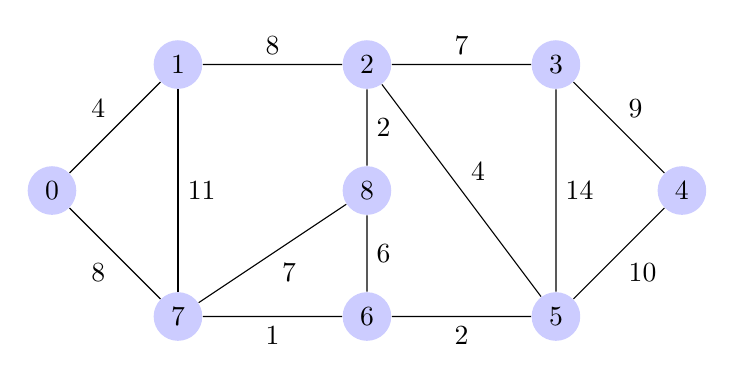
\begin{tikzpicture}
  [scale=.8,auto=left,every node/.style={circle,fill=blue!20}]
  \node (n0) at (-1,7) {0};
  \node (n1) at (1,9) {1};
  \node (n2) at (4,9) {2};
  \node (n3) at (7,9) {3};
  \node (n4) at (9,7) {4};
  \node (n5) at (7,5) {5};
  \node (n6) at (4,5) {6};
  \node (n7) at (1,5) {7};
  \node (n8) at (4,7) {8};  
  \foreach \from/\to /\pos in {n0/n1/4,n7/n0/8,n1/n2/8,n2/n3/7,n2/n5/4,n2/n8/2,n3/n4/9,n3/n5/14,n4/n5/10,n5/n6/2,n6/n7/1,n8/n6/6,n1/n7/11,n8/n7/7}
\tikzstyle{every node}=[ ]%%%%%%%%%%%%%%%%\tikzstyle{every node}=[fill=red!20]
    \draw (\from) -- (\to) node[midway]{\pos};
\end{tikzpicture}
\choice{۳۷}{۳۸}{۲۳}{۴۰}{a}
\begin{flushright}
\textbf{\color{red}پاسخ :}
\end{flushright}
گزینه الف صحیح می باشد:
{۳۷}

\begin{flushright}
\textbf{\color{green}حل :}
\end{flushright}
ابتدا تمامی یال ها را بر اساس وزن شان به صورت صعودی مرتب می کنیم سپس یال هارا به ترتیب انتخاب می کنیم به صورتی که حلقه ایجاد نشود.
\begin{latin}
{$1 + 2 + 2 + 4 + 4 + 7 + 8 + 9 = 37$}
\end{latin}

\vspace{0.1in}

%Question #13
\question
\vspace{0.1in}

%Question #14
\question
کدام الگوریتم برای یافتن کلیه کوتاه ترین مسیرها از مبدا واحدبه مقصدهای متفاوت به کارمی رود ؟
\choice{دایکسترا}{کروسکال}{پریم}{همه موارد}{a}
\begin{flushright}
\textbf{\color{red}پاسخ :}
\end{flushright}
گزینه الف صحیح می باشد:

{دایکسترا}

\begin{flushright}
\textbf{\color{green}حل :}
\end{flushright}
الگوریتم دایکسترا برای یافتن کلیه کوتاه ترین مسیرها از مبدأ واحد به مقصد های متفاوت به کار می رود. این الگوریتم هم چنین طول یک مسیر را برابر مجموع وزن یال های آن مسیر در نظر می گیرد.
\vspace{0.1in}

%Question #15
\question
\vspace{0.1in}

%Question #16
\question 
پیچیدگی زمانی الگوریتم حداقل ضرب ها به روش برنامه نویسی پویاکدام گزینه است ؟
\choice{$\theta(n^3)$}{$\theta(n^2)$}{$\theta(2^n)$}{$\theta(3^n)$}{a} %{e} Invalid answer choice
\begin{flushright}
\textbf{\color{red}پاسخ :}
\end{flushright}
گزینه الف صحیح می باشد:
{$\theta(n^3)$}

\begin{flushright}
\textbf{\color{green}حل :}
\end{flushright}
پیچیدگی زمانی الگوریتم حداقل ضرب ها {$\theta(n^3) $}
\vspace{0.1in}

%Question #17
\question
\vspace{0.1in}

%Question #18
\question 
پیچیدگی زمانی مسأله فروشنده دوره گرد با استفاده از برنامه نویسی پویا چیست ؟
\choice{$\theta(n^2)$}{$\theta(n^22^n)$}{$\theta(2^n)$}{$\theta(n^22^n\log n)$}{b} 
\begin{flushright}
\textbf{\color{red}پاسخ :}
\end{flushright}
گزینه ب صحیح می باشد:
{$\theta(n^22^n)$}

\begin{flushright}
\textbf{\color{green}حل :}
\end{flushright}
حل مسأله فروشنده دوره گرد به روش پویا دارای مرتبه زمانی {$n^22^n $} می باشد و میزان حافظه مورد نیاز {$n2^n$} است.
\vspace{0.1in}

%Question #19
\question
\vspace{0.1in}

%Question #20
\question
مسائلی که به روش بازگشت به عقب حل می شود چه نوع مسا‌‌ئلی هستند ؟
\choice{بهینه سازی}{تصمیم گیری}{تصمیم گیری وبهینه سازی}{هیچکدام}{b} 
\begin{flushright}
\textbf{\color{red}پاسخ :}
\end{flushright}
گزینه ب صحیح می باشد:

{تصمیم گیری}
\begin{flushright}
\textbf{\color{green}حل :}
\end{flushright}
مسائلی که به روش عقب گرد حل می شوند اغلب مسائل تصمیم گیری اند چون به راحتی توسط گراف و درخت می شوند:

روش عقب گرد در کاهش مرتبه زمانی تأثیر مثبت نمی گذارد.

روش عقب گرد حالت اصلاح شده جستجوی عمقی یک درخت است. 

روش عقب گرد ممکن است بیش از یک جواب داشته باشد همه جواب ها را باید پیدا کنیم.
\vspace{0.1in}

%Question #21
\question
\vspace{0.1in}

%Question #22
\question
مرتبه زمانی مسأله n وزیر کدام گزینه است ؟
\choice{n!}{$n^n$}{$n^2$}{$2^n$}{b} 
\begin{flushright}
\textbf{\color{red}پاسخ :}
\end{flushright}
گزینه ب صحیح می باشد:
{$n^n$}

\begin{flushright}
\textbf{\color{green}حل :}
\end{flushright}
در مساله {$n$} وزیر با توجه به درخت عقب گرد در سطح یک فقط یک گره وجود دارد و در سطح دو {$n$} گره و در سطح سوم {$n^2 $} و الی آخر پس برای بدست آوردن مرتبه زمانی آن به صورت زیر اقدام می کنیم:
\begin{latin}
{$ 1+ n + n^2 + n^3 + ... + n^n =\frac{n^(n+1)-1}{n-1} \in O(n^n) $}
\end{latin}
\vspace{0.1in}

%Question #23
\question
\vspace{0.1in}

%Question #24
\question
راه حل مسأله فروشنده دوره گرد در برنامه نویسی پویا و انشعاب و تحدید چه تفاوتی با هم دارد ؟
\choice
{با روش انشعاب وتحدید زمان اجرا کاهش می یابد.}   
{با روش انشعاب وتحدید حافظه مصرفی کاهش می یابد.}
{با روش انشعاب وتحدید مرتبه زمانی تغییر نمی کند .}
{روش برنامه نویسی پویا, زمان اجرا را کاهش می دهد .}{a}

\begin{flushright}
\textbf{\color{red}پاسخ :}
\end{flushright}
گزینه الف صحیح می باشد:

{با روش انشعاب وتحدید زمان اجرا کاهش می یابد.}  

\begin{flushright}
\textbf{\color{green}حل :}
\end{flushright}
مرتبه زمانی مسأله فروشنده دوره گرد با استفاده از روش پویا {$ O(n^22^n) $} می باشد. در روش انشعاب و تحدید با ارائه یک تابع حد مناسب زمان اجرای الگوریتم کاهش می یابد ولی مرتبه زمانی تغییری نمی کند.
\vspace{0.1in}

%Question #25
\question
\vspace*{\stretch{1}}
\newpage
\end{questions}

%%%%%%%%%%%%%%%%
%%%%%%%%%%%سوالات تشریحی
\begin{center}
\textbf{\color{blue}سوالات تشریحی زوج }
\end{center}

\begin{questions}
%Question #1
\question
\vspace*{1in}

%Question #2
\question
لیست زیر را به روش مرتب سازی ادغامی مرتب کنید (درخت فراخوانی های بازگشتی را رسم نموده و نحوه شکست لیست وادغام آنها را نمایش دهید ):
\begin{latin}
\begin{lstlisting}
12 5 7 13 56 90 1 3 9
\end{lstlisting}
\end{latin}
\begin{flushright}
\textbf{\color{red}پاسخ :}
\end{flushright}

\begin{latin}
\begin{center}
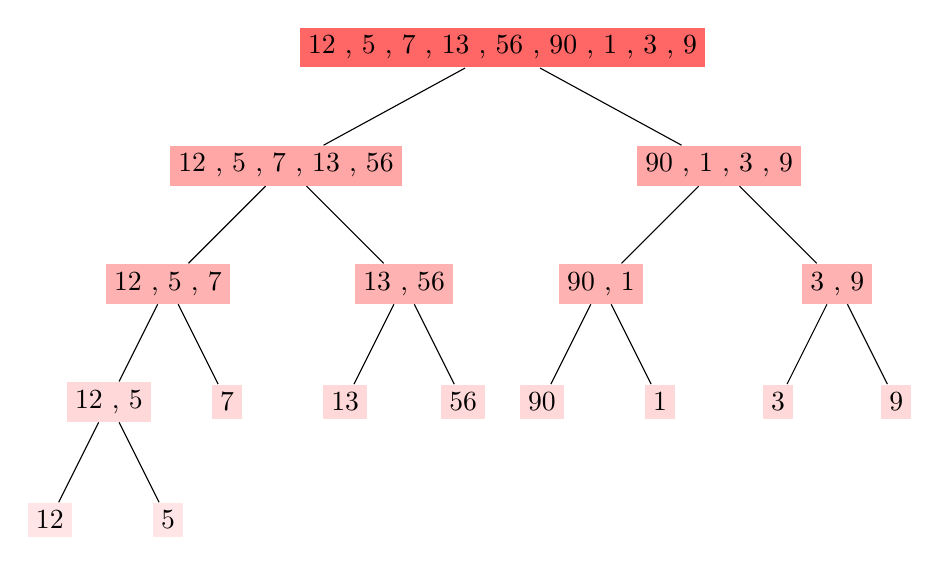
\begin{tikzpicture}[level distance=15mm]
\tikzstyle{every node}=[fill=red!60,rectangle,inner sep=3pt]
\tikzstyle{level 1}=[sibling distance=55mm,
set style={{every node}+=[fill=red!35]}]
\tikzstyle{level 2}=[sibling distance=30mm,
set style={{every node}+=[fill=red!30]}]
\tikzstyle{level 3}=[sibling distance=15mm,
set style={{every node}+=[fill=red!15]}]
\tikzstyle{level 4}=[sibling distance=15mm,
set style={{every node}+=[fill=red!10]}]
\node {12 , 5 , 7 , 13 , 56 , 90 , 1 , 3 , 9}
child {node {12 , 5 , 7 , 13 , 56}
child {node {12 , 5 , 7}
child {node {12 , 5}
child {node {12}}
child {node {5}}
}
child {node {7}}
}
child {node {13 , 56}
child {node {13}}
child {node {56}}
}
}
child {node {90 , 1 , 3 , 9}
child {node {90 , 1}
child {node {90}}
child {node {1}}
}
child {node {3 , 9}
child {node {3}}
child {node {9}}
}
};
\end{tikzpicture}
\end{center}
\end{latin}


\vspace{0.5in}

%Question #3
\question
\vspace*{1in}



%Question #4
\question
ماتریس های زیر را در نظر بگیرید :
\begin{latin}
$A_{3\times4}$\\
$B_{4\times8}$\\
$C_{8\times3}$\\
$D_{3\times5}$
\end{latin}
چنانچه بخواهیم تعداد ضربها برای به دست آوردن حاصل ضرب {$A\times B \times C \times D$} را به روش برنامه نویسی پویا به دست آوریم, محاسبات مربوطه را به صورت کاملاً مشروح نوشته و محاسبه نمائید. (ماتریس محاسبات مربوطه را تشکیل دهید و اعداد محاسبه شده در هر مرحله را در ماتریس قرار دهید )

\begin{flushright}
\textbf{\color{red}پاسخ :}
\end{flushright}
با توجه به فرمول روش پویا جدول مربوطه را کامل می کنیم:
\begin{latin}
{$ m1 = min( m_{1k} +m_{k+1j} + r_{i-1} \times r_{k} \times r_{j} ) \quad i \leq k < j \\
    m_{11} = m_{22} = m_{33} = m_{44} = 0 \\
    m_{12} = min ( m_{11} + m_{22} + 3 \times 4 \times 8 )=96 \\
    m_{23} = min ( m_{22} + m_{33} + 4 \times 8 \times 3 )=96\\
    m_{34} = min ( m_{33} + m_{44} + 8 \times 3 \times 4 )=120 \\
    m_{13} = min ( m_{11} + m_{23} + 3 \times 4 \times 3 , m_{12} + m_{33} + 3 \times 8 \times 3 )= min(132 , 168) = 13\\
m_{24} = min ( m_{22} + m_{34} + 4 \times 8 \times 5 , m_{23} + m_{44} + 4 \times 3 \times 5 )= min(280 , 156) = 15\\
m_{14} = min ( m_{11} + m_{24} + 3 \times 4 \times 5 , m_{12} + m_{34} + 3 \times 8 \times 5 , m_{13} + m_{44} +3 \times 3 \times 5 )= min(216 , 240 , 177) = 177
$}


\end{latin}
\vspace{0.5in}

%Question #5
\question
\vspace*{\stretch{1}}
\newpage

\end{questions}

%%%%%%%%%%%%%%%%%
%\newpage  %Uncomment to put on new age

\bigskip
\begin{center}
\textbf{\color{blue} پاسخ سوالات تستی زوج }
\end{center}
\bigskip  

\showallanswers % 

\end{document}

